\subsection{Emulator}

The purpose of any \ac{isa} is, at its core, to execute software written for it. As explained in \autoref{sec:isa_vs_implementation}, an \ac{isa} by itself cannot execute code; an implementation is required to do so. This implementation can be done either in hardware or in software. Although the end goal of this work is to have a hardware implementation, software is far more maleable and therefore easier to create and modify. For this reason, to test and verify design choices made during the \ac{isa} design process, a software implementation is built. This software then emulates the behavior of the \ac{isa}, hence it is called an ``emulator'' of said architecture.

\subsubsection{Logic gate simulation}

Since the hardware shall be built from individual logic gates, the software emulator should reflect this to make the gap from the tested system to the hardware system as small as possible. This minimizes the errors introduced translating from one level of abstraction to another. To implement such a simulation, the digital logic simulator ``Digital'' by Heinz Neemann is used \cite{neemann_digital}. It is free to use and well documented and was previously used by the author to simulate other logical circuits. For these reasons, the cost of entry in both money and time spent learning to use the tool are minimal. The tool simulates digital logic circuits, which can then be hierarchically combined to form more and more complex circuits. \autoref{fig:digital_full_adder} shows a circuit that implements a 1 bit full adder within the software. \autoref{fig:digital_full_adder_reuse} shows how this circuit can then be reused in higher-level circuits.

\begin{figure}[h!]
    \centering
    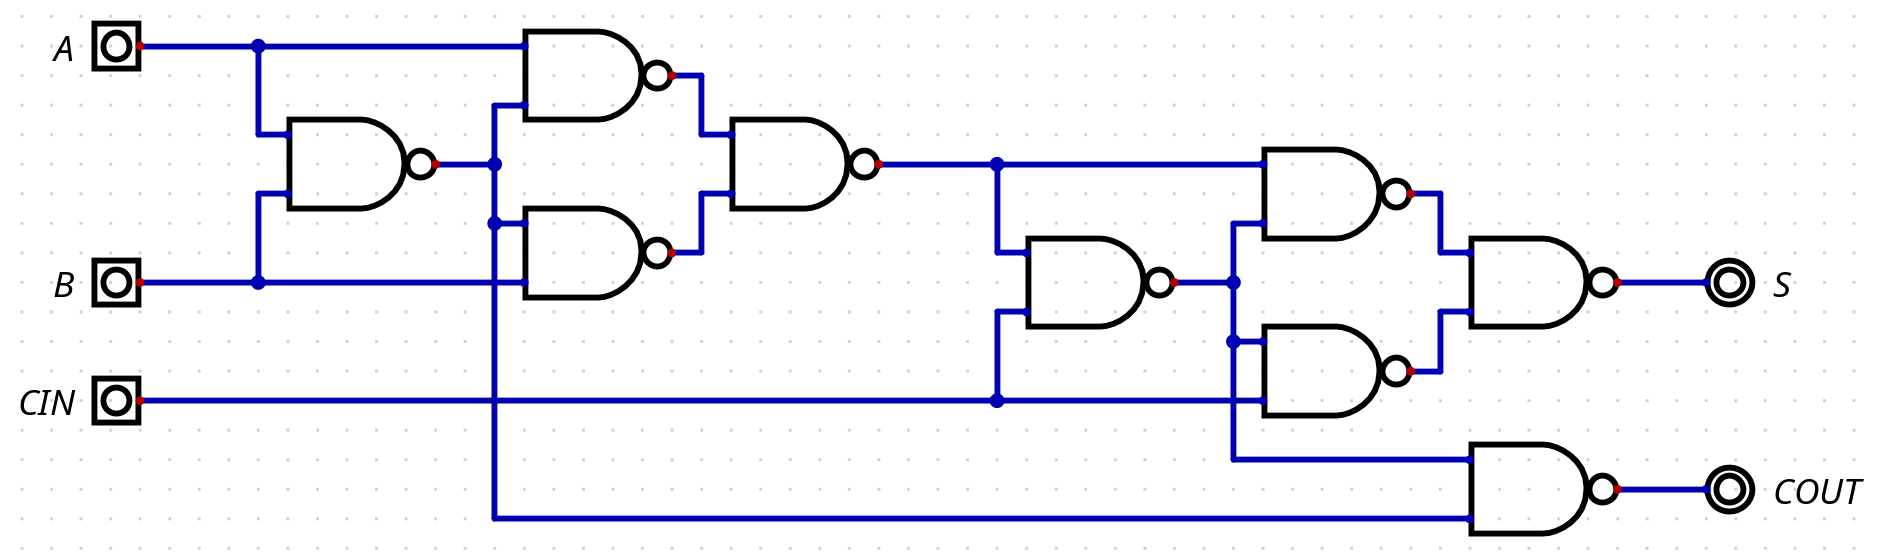
\includegraphics[width=0.8\textwidth]{images/digital_full_adder.png}
    \caption{1 Bit full adder in the logic gate simulator ``Digital''}
    \label{fig:digital_full_adder}
\end{figure}

\begin{figure}[h!]
    \centering
    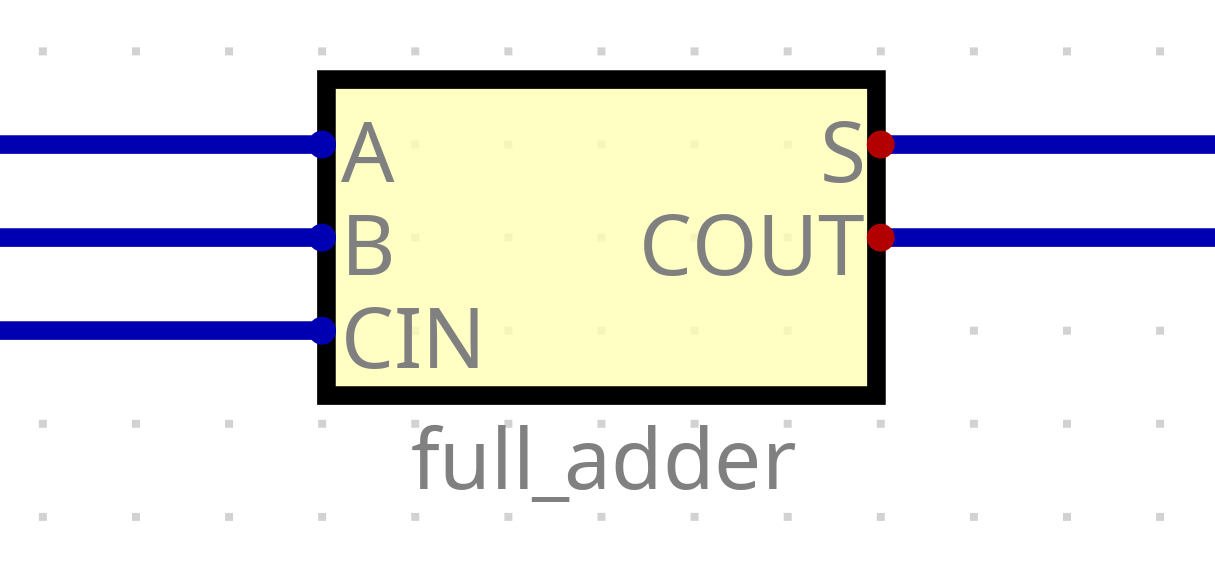
\includegraphics[width=0.8\textwidth]{images/digital_full_adder_reuse.png}
    \caption{Hierarchical reuse of the 1 bit full adder shown in \autoref{fig:digital_full_adder}}
    \label{fig:digital_full_adder_reuse}
\end{figure}

This hierarchical nesting of circuit implementations allows for easier management of large numbers of gates, as well as reuse of common components. For example, 8 instances of the same 1 bit full adder can be connected to form an 8 bit word full adder. This approach of nesting also naturally leads to better semantic grouping of circuits, which can later be reused to divide the hardware implementation into reasonably sized \acp{pcb}.

\subsubsection{State transition}

The emulator must have a smallest, atomic unit of execution. Since the \ac{cpu} operates on the standard fetch, decode execute instruction cycle, this can be chosen to be either a single phase, or an integer number of instruction cycles. 